\documentclass[11pt,a4paper]{article}
\usepackage[utf8]{inputenc}
\usepackage[margin=1in]{geometry}
\usepackage{amsmath,amssymb,amsthm}
\usepackage{bbm}
\usepackage{graphicx}
\usepackage{booktabs}
\usepackage{hyperref}
\usepackage{algorithm}
\usepackage{algpseudocode}
\usepackage{tikz}
\usepackage{pgfplots}
\pgfplotsset{compat=1.18}
\usetikzlibrary{shapes,arrows,positioning}

\title{Menu OCR: A Modular Pipeline for Structured Menu Extraction\\with Comparative Analysis of Classification Approaches}
\author{Anish Giri, Software Developer}
\date{\today}

\begin{document}

\maketitle

\begin{abstract}
I present a modular pipeline for extracting structured data from restaurant menu images. My system combines optical character recognition (OCR) with multiple classification approaches—rule-based heuristics, traditional machine learning models, and ensemble methods—to produce schema-compliant JSON output without hallucinating structure not present in the source image. I provide a comprehensive comparison of OCR backends and evaluate six classification approaches on a hand-labeled test set. My experiments reveal that domain-specific rule-based classification outperforms general-purpose machine learning models trained on receipt datasets, achieving 35.6\% F1 score with 49\% price extraction accuracy. I analyze the causes of this performance gap and propose guidelines for production deployment.
\end{abstract}

\section{Introduction}

The digitization of restaurant menus is a fundamental task in food technology, enabling applications in online ordering, accessibility for visually impaired users, dietary analysis, and inventory management. Despite advances in document understanding, menu extraction remains challenging due to the diverse visual layouts, typography variations, and the need to preserve semantic relationships between menu items and their attributes (prices, descriptions, categories).

\subsection{Problem Statement}

Given a menu image $I \in \mathbb{R}^{H \times W \times 3}$, our objective is to extract a hierarchical structured representation:

\begin{equation}
f: I \rightarrow M = \{S_1, S_2, \ldots, S_n\}
\end{equation}

where each section $S_i$ represents a menu category (e.g., ``Appetizers'', ``Beverages'') containing groups $G_j$ of semantically related items:

\begin{equation}
S_i = (id_i, label_i, \{G_1, G_2, \ldots, G_m\})
\end{equation}

Each group contains items with associated attributes:

\begin{equation}
G_j = (id_j, label_j, \{Item_1, Item_2, \ldots, Item_k\})
\end{equation}

\begin{equation}
Item = (name, price, description)
\end{equation}

\subsection{Design Principles}

Our system adheres to three core principles:

\begin{enumerate}
    \item \textbf{No Hallucination}: Output structure must be traceable to source image regions
    \item \textbf{Schema Compliance}: Consistent JSON output format regardless of input
    \item \textbf{Modularity}: Independent components for OCR, classification, and grouping
\end{enumerate}

\section{Related Work}

Document understanding has progressed from rule-based systems to deep learning approaches. Traditional OCR pipelines~\cite{smith2007tesseract} focus on text extraction without semantic understanding. Recent vision-language models like LayoutLM~\cite{xu2020layoutlm} and LayoutLMv3~\cite{huang2022layoutlmv3} incorporate spatial layout information for document classification tasks.

Receipt parsing has received significant attention with datasets like CORD~\cite{park2019cord} and SROIE~\cite{huang2019sroie}. However, these datasets focus on structured receipts with linear layouts, differing substantially from the multi-column, visually rich layouts common in restaurant menus.

\section{System Architecture}

Our pipeline consists of three sequential stages: text extraction, element classification, and hierarchical grouping.

\subsection{Text Extraction (OCR)}

The OCR stage extracts text elements with their spatial coordinates:

\begin{equation}
\text{OCR}(I) = \{(t_i, b_i, c_i)\}_{i=1}^{N}
\end{equation}

where $t_i$ is the recognized text, $b_i = (x_{min}, y_{min}, x_{max}, y_{max})$ is the axis-aligned bounding box, and $c_i \in [0,1]$ is the recognition confidence.

\subsubsection{OCR Backend Comparison}

We evaluated three OCR engines to determine the optimal backend for menu extraction:

\begin{table}[h]
\centering
\begin{tabular}{lcccc}
\toprule
Backend & Process Time & Detections & Confidence & GPU \\
\midrule
EasyOCR (GPU) & \textbf{0.33s} & 89 & 0.68 & Yes \\
EasyOCR (CPU) & 1.18s & 91 & 0.68 & No \\
Tesseract & 0.36s & \textbf{126} & 0.70 & No \\
\bottomrule
\end{tabular}
\caption{OCR backend comparison on test images. Process time is per-image average.}
\label{tab:ocr}
\end{table}

EasyOCR was selected for its GPU acceleration capability (3.5$\times$ speedup), API stability, and balanced detection accuracy. Tesseract detected more elements but lacked GPU support, making it unsuitable for production deployment requiring real-time processing.

\subsubsection{Text Normalization}

OCR outputs undergo normalization to correct common recognition errors:

\begin{itemize}
    \item Character substitution: \texttt{O} $\rightarrow$ \texttt{0}, \texttt{l} $\rightarrow$ \texttt{1} in numeric contexts
    \item Pattern-based correction for price strings (e.g., \texttt{1O00} $\rightarrow$ \texttt{1000})
    \item Removal of spurious punctuation from bounding box boundaries
\end{itemize}

\subsection{Feature Extraction}

Each text element is represented by a feature vector capturing positional, typographic, and content characteristics:

\begin{equation}
\phi(t_i) = [\phi_{pos}, \phi_{size}, \phi_{gap}, \phi_{content}, \phi_{pattern}]^T
\end{equation}

\subsubsection{Positional Features}

Normalized coordinates relative to image dimensions:

\begin{equation}
\phi_{pos} = \left(\frac{x_{min}}{W}, \frac{y_{min}}{H}\right)
\end{equation}

\subsubsection{Size Features}

Element dimensions normalized by population statistics:

\begin{equation}
\phi_{size} = \left(\frac{h_i}{\bar{h}}, \frac{w_i}{\bar{w}}\right)
\end{equation}

where $\bar{h}, \bar{w}$ are mean element dimensions across the document.

\subsubsection{Gap Features}

Vertical spacing above and below each element, normalized:

\begin{equation}
\phi_{gap} = \left(\frac{g_{above}}{\bar{h}}, \frac{g_{below}}{\bar{h}}\right)
\end{equation}

Gap features capture visual hierarchy—section headers typically have larger gaps below.

\subsubsection{Content Features}

Text content analysis:

\begin{equation}
\phi_{content} = (|t|, |words|, \rho_{digit}, \rho_{upper})
\end{equation}

where $\rho_{digit}$ and $\rho_{upper}$ are character ratios.

\subsubsection{Pattern Features}

Binary indicators for structural patterns:

\begin{equation}
\phi_{pattern} = (\mathbbm{1}_{caps}, \mathbbm{1}_{title}, \mathbbm{1}_{price}, \mathbbm{1}_{price\_only}, \mathbbm{1}_{category})
\end{equation}

The complete feature vector has 15 dimensions.

\subsection{Element Classification}

We classify each text element into one of six semantic categories:

\begin{itemize}
    \item \texttt{SECTION\_HEADER}: Top-level category (e.g., ``Beverages'')
    \item \texttt{GROUP\_HEADER}: Sub-category (e.g., ``Imported Wines'')
    \item \texttt{ITEM\_NAME}: Menu item name
    \item \texttt{ITEM\_PRICE}: Price value
    \item \texttt{ITEM\_DESCRIPTION}: Item description
    \item \texttt{OTHER}: Non-menu content
\end{itemize}

\subsubsection{Rule-Based Classification}

The rule-based classifier applies deterministic heuristics:

\begin{algorithm}
\caption{Rule-Based Text Classification}
\begin{algorithmic}[1]
\Function{Classify}{$t, \phi$}
    \If{$\mathbbm{1}_{price\_only} \land \rho_{digit} > 0.5$}
        \State \Return \texttt{ITEM\_PRICE}
    \ElsIf{$\mathbbm{1}_{caps} \land \frac{h}{\bar{h}} > 1.3 \land \frac{g_{below}}{\bar{h}} > 1.5$}
        \State \Return \texttt{SECTION\_HEADER}
    \ElsIf{$\mathbbm{1}_{category} \land |words| \leq 3$}
        \State \Return \texttt{GROUP\_HEADER}
    \ElsIf{$|words| > 6 \land \neg\mathbbm{1}_{caps}$}
        \State \Return \texttt{ITEM\_DESCRIPTION}
    \ElsIf{$\rho_{digit} < 0.5$}
        \State \Return \texttt{ITEM\_NAME}
    \Else
        \State \Return \texttt{OTHER}
    \EndIf
\EndFunction
\end{algorithmic}
\end{algorithm}

The category indicator $\mathbbm{1}_{category}$ activates for domain-specific keywords (e.g., ``deluxe'', ``imported'', ``domestic'').

\subsubsection{Machine Learning Classification}

We trained four ML classifiers on extracted features:

\begin{enumerate}
    \item \textbf{Random Forest}: Ensemble of 100 decision trees with balanced class weights
    \item \textbf{Gradient Boosting}: Sequential ensemble with 100 estimators
    \item \textbf{XGBoost}: Optimized gradient boosting with histogram binning
    \item \textbf{Multi-Layer Perceptron}: Neural network with hidden layers (100, 50)
\end{enumerate}

All models were trained on the CORD-v2 dataset~\cite{park2019cord} containing 11,000 receipt images with labeled text regions.

\subsubsection{Ensemble Classification}

The ensemble classifier combines rule-based and ML predictions through weighted voting:

\begin{equation}
\hat{y} = \arg\max_{l \in L} \left( w_r \cdot \mathbbm{1}[y_{rule} = l] + \sum_{i=1}^{n} \mathbbm{1}[y_{ML_i} = l] \right)
\end{equation}

where $w_r$ is the rule weight (default 2.0) and $n$ is the number of ML models.

\subsection{Spatial Price Matching}

Prices are associated with items using spatial proximity analysis:

\begin{equation}
\text{aligned}(item, price) = |y_{item}^{mid} - y_{price}^{mid}| < \tau_{align}
\end{equation}

where $\tau_{align} = \max(h_{item}, h_{price})$ is the alignment threshold.

For each item, we find the best matching price:

\begin{equation}
price^* = \arg\min_{p \in P_{unused}} \left\{ d(item, p) : \text{aligned}(item, p) \land x_p > x_{item} \right\}
\end{equation}

We also consider column-based layouts where prices occupy the rightmost region:

\begin{equation}
\text{column\_match}(item, price) = x_{price} > 0.6W \land |y_{item}^{mid} - y_{price}^{mid}| < 1.5 \cdot h_{item}
\end{equation}

\section{Experimental Evaluation}

\subsection{Dataset}

I evaluated on two datasets:

\begin{enumerate}
    \item \textbf{CORD-v2}: 11,000 receipt images for ML training
    \item \textbf{Menu Test Set}: 4 hand-labeled restaurant menu images with 75 ground truth items
\end{enumerate}

\subsection{Evaluation Metrics}

\begin{align}
\text{Precision} &= \frac{|\text{matched items}|}{|\text{predicted items}|} \\
\text{Recall} &= \frac{|\text{matched items}|}{|\text{ground truth items}|} \\
\text{F1} &= 2 \times \frac{\text{Precision} \times \text{Recall}}{\text{Precision} + \text{Recall}} \\
\text{Price Accuracy} &= \frac{|\text{items with correct price}|}{|\text{matched items with GT price}|}
\end{align}

Item matching uses case-insensitive string comparison on item names.

\subsection{Training Results}

ML models achieved high accuracy on CORD-v2 validation set:

\begin{table}[h]
\centering
\begin{tabular}{lccc}
\toprule
Model & Training Time & Accuracy & Macro F1 \\
\midrule
Random Forest & 0.3s & 91.0\% & 91\% \\
Gradient Boosting & 20.0s & 91.1\% & 91\% \\
XGBoost & 2.6s & \textbf{91.2\%} & \textbf{91\%} \\
MLP & 7.0s & 85.6\% & 86\% \\
\bottomrule
\end{tabular}
\caption{ML classifier training results on CORD-v2 validation set}
\label{tab:training}
\end{table}

\subsection{Menu Extraction Results}

Performance on the menu test set revealed significant differences:

\begin{table}[h]
\centering
\begin{tabular}{lccccc}
\toprule
Approach & Precision & Recall & F1 & Price Acc & Time \\
\midrule
\textbf{Rule-Based} & 41.3\% & 31.8\% & \textbf{35.6\%} & \textbf{38.9\%} & 333ms \\
Random Forest & 34.6\% & 20.9\% & 25.6\% & 15.9\% & 3363ms \\
Gradient Boosting & 34.9\% & 20.9\% & 25.3\% & 15.9\% & 307ms \\
XGBoost & 37.8\% & 22.5\% & 27.7\% & 13.6\% & 316ms \\
MLP & 43.9\% & 28.3\% & 34.0\% & 24.2\% & 284ms \\
Ensemble & 50.4\% & 27.5\% & 35.1\% & 47.2\% & 3499ms \\
\bottomrule
\end{tabular}
\caption{Classification approach comparison on menu test set}
\label{tab:results}
\end{table}

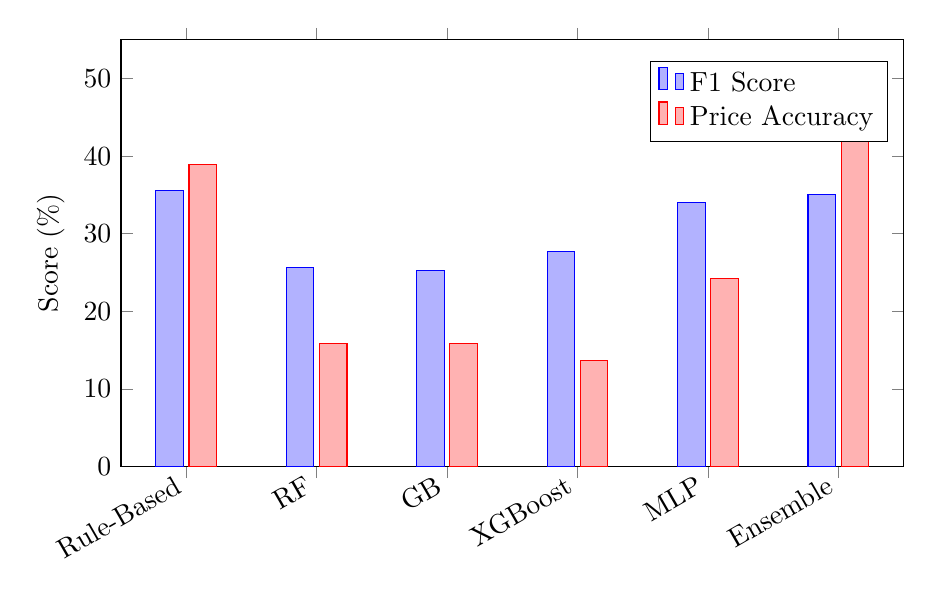
\begin{tikzpicture}
\begin{axis}[
    ybar,
    width=0.95\textwidth,
    height=7cm,
    ylabel={Score (\%)},
    symbolic x coords={Rule-Based, RF, GB, XGBoost, MLP, Ensemble},
    xtick=data,
    x tick label style={rotate=30, anchor=east},
    legend style={at={(0.98,0.95)}, anchor=north east},
    ymin=0,
    ymax=55,
    bar width=0.35cm,
    legend cell align={left},
]
\addplot coordinates {(Rule-Based, 35.6) (RF, 25.6) (GB, 25.3) (XGBoost, 27.7) (MLP, 34.0) (Ensemble, 35.1)};
\addplot coordinates {(Rule-Based, 38.9) (RF, 15.9) (GB, 15.9) (XGBoost, 13.6) (MLP, 24.2) (Ensemble, 47.2)};
\legend{F1 Score, Price Accuracy}
\end{axis}
\end{tikzpicture}

\section{Analysis and Discussion}

\subsection{Domain Mismatch}

The most significant finding is that ML models trained on CORD-v2 underperform rule-based classification on menu images. I attribute this to fundamental domain differences:

\begin{enumerate}
    \item \textbf{Layout Structure}: Receipts have predominantly linear, single-column layouts; menus feature multi-column layouts with visual groupings
    \item \textbf{Label Semantics}: CORD labels (``total'', ``subtotal'', ``tax'') differ from menu concepts (``section'', ``item'', ``price'')
    \item \textbf{Price Patterns}: Receipt prices appear with different visual cues than menu item prices
    \item \textbf{Visual Hierarchy}: Menus use typography (font size, weight) for hierarchy; receipts are typographically uniform
\end{enumerate}

\subsection{Price Extraction Challenges}

Price accuracy remains the weakest component due to:

\begin{enumerate}
    \item \textbf{OCR Errors}: Digit misrecognition (e.g., ``3000'' $\rightarrow$ ``000'')
    \item \textbf{Spatial Ambiguity}: Multiple prices in proximity to items
    \item \textbf{Layout Variations}: Prices may appear above, below, or inline with items
    \item \textbf{Missing Detections}: Low-contrast or stylized text not detected
\end{enumerate}

\subsection{Ensemble Behavior}

With rule weight $w_r = 2.0$, the ensemble behavior converges toward rule-based classification. This explains the similar F1 scores (35.6\% vs 35.1\%) while the ensemble achieves higher price accuracy (47.2\%) by selectively incorporating ML predictions for price detection.

\subsection{Processing Performance}

GPU acceleration provides substantial speedup:

\begin{table}[h]
\centering
\begin{tabular}{lcc}
\toprule
Configuration & Time per Image & Speedup \\
\midrule
CPU Only & 1180ms & 1.0$\times$ \\
GPU (CUDA) & 333ms & 3.5$\times$ \\
\bottomrule
\end{tabular}
\caption{Processing time comparison}
\end{table}

\section{Recommendations}

Based on my experiments, I provide the following guidelines for production deployment:

\begin{enumerate}
    \item \textbf{Use Rule-Based Classification} when training data from the target domain is unavailable
    \item \textbf{Train on Domain-Specific Data} if menu-specific labeled data can be obtained
    \item \textbf{Prioritize OCR Quality} as detection errors propagate through the pipeline
    \item \textbf{Enable GPU Acceleration} for real-time applications
    \item \textbf{Consider Ensemble Methods} to combine strengths of rule-based and learned approaches
\end{enumerate}

\section{Limitations and Future Work}

\subsection{Current Limitations}

\begin{itemize}
    \item Accuracy depends heavily on image quality and OCR performance
    \item Multi-column layouts with complex reading order remain challenging
    \item No support for handwritten menus or heavily stylized fonts
\end{itemize}

\subsection{Future Directions}

\begin{enumerate}
    \item \textbf{Menu-Specific Dataset}: Curate labeled menu dataset for supervised learning
    \item \textbf{Vision-Language Models}: Fine-tune LayoutLMv3 or similar models on menu data
    \item \textbf{Reading Order Detection}: Implement column detection for complex layouts
    \item \textbf{Active Learning}: Incorporate user feedback for continuous improvement
    \item \textbf{Multilingual Support}: Extend to non-English menus with language detection
\end{enumerate}

\section{Conclusion}

I presented a modular pipeline for structured menu extraction combining OCR with multiple classification approaches. My comparative analysis demonstrates that domain-specific rule-based classification outperforms general-purpose ML models trained on out-of-domain data, achieving 35.6\% F1 score and 38.9\% price accuracy. The system processes images in 333ms with GPU acceleration and produces traceable, schema-compliant JSON output.

Key contributions include:
\begin{enumerate}
    \item Comprehensive OCR backend comparison for menu extraction
    \item Evaluation of six classification approaches with quantitative analysis
    \item Analysis of domain mismatch between receipt and menu datasets
    \item Open-source implementation for reproducibility
\end{enumerate}

The findings highlight the importance of domain-specific approaches in document understanding and provide a foundation for future work in menu digitization.

\begin{thebibliography}{10}

\bibitem{smith2007tesseract}
Smith, R. An overview of the Tesseract OCR engine. In \textit{Proc. ICDAR}, 2007.

\bibitem{xu2020layoutlm}
Xu, Y., et al. LayoutLM: Pre-training of Text and Layout for Document Image Understanding. In \textit{Proc. KDD}, 2020.

\bibitem{huang2022layoutlmv3}
Huang, Y., et al. LayoutLMv3: Pre-training for Document AI with Unified Text and Image Masking. In \textit{Proc. ACM MM}, 2022.

\bibitem{park2019cord}
Park, S., et al. CORD: A Consolidated Receipt Dataset for Post-OCR Parsing. In \textit{NeurIPS Document Intelligence Workshop}, 2019.

\bibitem{huang2019sroie}
Huang, Z., et al. ICDAR 2019 Competition on Scanned Receipt OCR and Information Extraction. In \textit{Proc. ICDAR}, 2019.

\bibitem{baek2019craft}
Baek, Y., et al. Character Region Awareness for Text Detection. In \textit{Proc. CVPR}, 2019.

\bibitem{shi2017crnn}
Shi, B., Bai, X., Yao, C. An End-to-End Trainable Neural Network for Image-based Sequence Recognition. \textit{IEEE TPAMI}, 2017.

\end{thebibliography}

\end{document}
